\PassOptionsToPackage{dvipsnames}{xcolor}
\documentclass{beamer}
\usepackage{xcolor}
\usepackage{pgfpages}

\usepackage[style=authortitle]{biblatex}

\setbeameroption{show notes on second screen}

\usepackage[utf8]{inputenc}
\usepackage[T1]{fontenc}
\usepackage{lmodern}
\usepackage{fontawesome}

\usepackage{minted}

\usepackage{listings}

\usepackage[american]{babel}

\usepackage{
    amsmath,
    amsfonts,
    amssymb
}

\usepackage[os=win]{menukeys}

\usetheme{UOS}

\graphicspath{{img/}}

% use this with \begin{pythoncode} ... \end{pythoncode}
\newminted{python}{linenos=false}

\newminted[outputcode]{text}{linenos=false}

% this gets rid of red boxes around syntax errors in minted
\AtBeginEnvironment{minted}{%
  \renewcommand{\fcolorbox}[4][]{#4}}

% removes the prefix "Figure 1:" in figure captions
\setbeamertemplate{caption}{\raggedright\insertcaption\par}

\usepackage{gensymb}
\usepackage{csquotes}
\usepackage{fontawesome}

\nocite{*}
\addbibresource{references.bib}

\begin{document}

\title[Introduction]{Week 1: Introduction}
\subtitle{Basic Programming in Python}

\author[jwippermann, rhorn, kvatankhahba, lfrommelt]{Julia Wippermann, Robin Horn, Kamran Vatankhah-Barazandeh, Leonard Frommelt}

% change to date of actual lecture
\date{\today}

\begin{frame}[plain]
    \titlepage
\end{frame}

\begin{frame}
    \tableofcontents
\end{frame}

\section{About this course}

\subsection{Who we are}

\begin{frame}{Who we are}

    \begin{enumerate}
        \item Julia Wippermann (jwippermann@uos.de):
        \newline 2nd Semester Info Master / Bachelor Lehramt
        \newline
        \item Robin Horn (rhorn@uos.de):
        \newline 6th Semester CogSci
        \item Kamran Vatankhah-Barazandeh (kvatankhahba@uos.de):
        \newline 6th Semester CogSci
        \newline
        \item Leonard Frommelt (lfrommelt@uos.de):
        \newline 10th Semester CogSci Bachelor
    \end{enumerate}
\end{frame}

\subsection{Who should attend this Course}

\begin{frame}{Who this course is for}

    You are in the right course if...
    \newline
    \begin{enumerate}[a]
        \item You are a master student coming from a non-technical discipline
        \item You have little to no experience with programming
        \item You felt a little overwhelmed by Informatik A and would like to repeat the core principles of programming with another language
    \end{enumerate}

\end{frame}

\begin{frame}{Who this course is for}

    You are NOT in the right course if...
    \newline
    \begin{enumerate}[a]
        \item Informatik A was a piece of cake for you and you would just like to learn another language
        \newline $\rightarrow$ Scientific Programming in Python
        \item You already know Python and would like to earn an easy good grade
        \newline $\rightarrow$ ECTS will be gradeless
        \item You have a specific application area that you want to learn about in detail
        \newline $\rightarrow$ Specialized courses (CV, CL, ML etc.)
    \end{enumerate}

\end{frame}

\subsection{Schedule}

\begin{frame}{Tentative Schedule}

    \begin{enumerate}
        \item Hello World
        \item Variables \& Assignments
        \item Control Structures
        \item Data Structures
        \item Strings \& Formatting
        \item Input \& Output
        \item Debugging \& Good Practices
        \item Built-In Packages
        \item Object-Oriented Programming
    \end{enumerate}
    $\rightarrow$ More lectures on external packages %\newline
    $\rightarrow$ Working on projects

\end{frame}

\subsection{Structure}

\begin{frame}{Structure}

    \begin{enumerate}
        \item Lecture:
        \newline Tuesday 12:15 - 13:45 in 66/E33
        \item Walk-In Practice Session:
        \newline Thursday 12:15 - 13:45 in 66/E33
        \item Homework Submission:
        \newline Until Sunday 23:59:59 via StudIP
        \item Feedback:
        \newline We'll arrange a meeting if requested
    \end{enumerate}

    \note{
        \begin{itemize}
            \item \textbf{Lecture:} We will introduce new topics here
            \item \textbf{Walk-In:} You can come and work on your homework assignments. It should be a nice working atmosphere and you can get help if you are stuck!
            \item \textbf{Feedback:} You can get individual feedback on your homework submission
        \end{itemize}
    }

\end{frame}

\begin{frame}{Homework and Grading}

    \begin{alertblock}{\textbf{Homework Regulations}}
    \begin{enumerate}
        \item One homework sheet per week (12 in total)
        \item One passed homework sheet worth 1 point
        \item Sheet submission in groups of 2-4 via StudIP groups
        \item Optional project in the end worth 2-3 points
        \item \textbf{At least 10 points are required to pass the course}
    \end{enumerate}
    \end{alertblock}

\end{frame}

\begin{frame}{Homework Groups}

    \begin{enumerate}
        \item There are around 30 homework groups available
        \item In each group there should be 3-4 students
        \item You can enter a group between 18:00 today and Sunday
    \end{enumerate}

    \vspace{1em}

    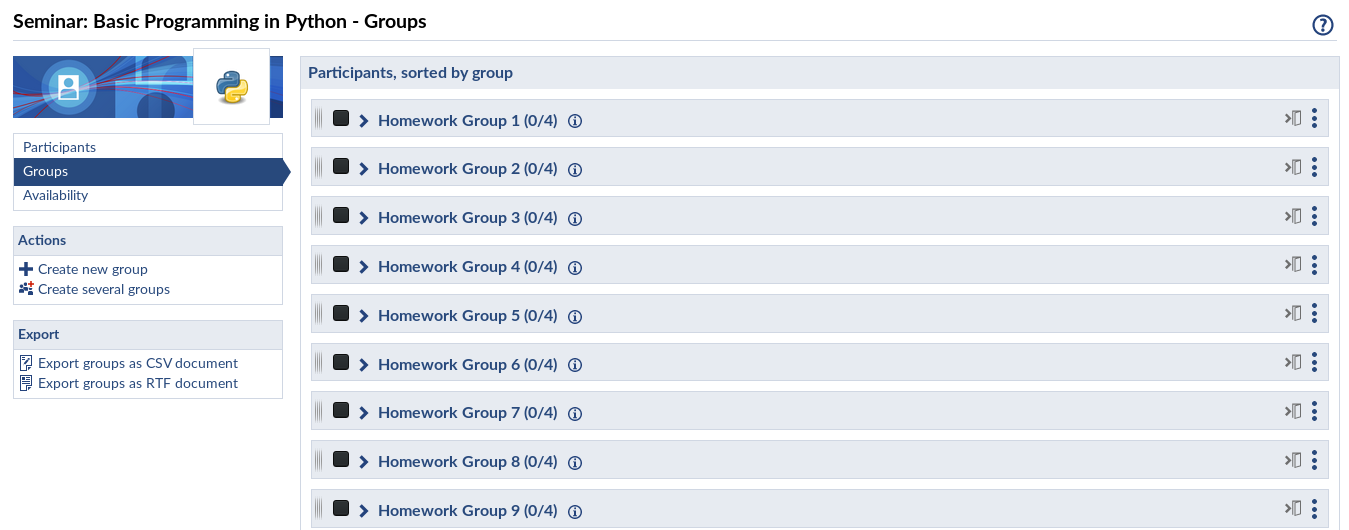
\includegraphics[width=\textwidth]{groups.png}

\end{frame}

\section{What is programming?}

\subsection{Why Coxies need Programming}
%By now playground

\begin{frame}{Some Examples}

    \begin{itemize}
        \item <2-> \textbf{Visualizing Data} \\
        here could be a nice pyplot example

        \item <3-> \textbf{Machine Learning} \\
        Artificial Neural Networks, Reinforcement learning, Computer Vision, etc...

        \item <4-> \textbf{And a few more selected Examples} \\
        Statistics, automatisation, surveys, ...
    \end{itemize}

    \pause

    \vspace{0.5cm}

    \uncover<5->{\textbf{Some sort of conclusion or whatever}}

    \vspace{0.5cm}

    \note{
        \begin{itemize}
            \item \textit{italic note}, more notes, ..., \textbf{fat note}
        \end{itemize}
        \begin{itemize}
            \item second note section
        \end{itemize}
    }

\end{frame}

\subsection{Algorithms}

\begin{frame}{What is an Algorithm?}

    \begin{alertblock}{\textbf{Definition}}
        [...] an \textit{Algorithm} is an \textbf<3>{unambiguous} \textbf<2>{specification} of how to solve a \textbf<4>{class of problems}. \footfullcite{wiki:algorithm}
    \end{alertblock}

    \begin{itemize}
        \item <2-> \textbf{specification} \\
        meaning a description / instructions

        \item <3-> \textbf{unambiguous} \\
        at each point you know exactly what the next step is

        \item <4-> \textbf{problem-specific} \\
        an algorithm for sheering sheep won't help milking cows
    \end{itemize}

    \vspace{0.5cm}

    \uncover<5->{\textbf{Example:} A cooking recipe}

    \vspace{0.5cm}

    \note{
        \begin{itemize}
            \item \textit{Problem-specific} is fairly loosely used here: If it only solves \textbf{one} specific problem, we might as well just memorize the solution. But of course, we cannot have a general algorithm for \textbf{all} problems. Good classes of problems are somewhere inbetween, like sorting an \textbf{arbitrary list of numbers} in ascending order.
        \end{itemize}
    }

\end{frame}

\subsection{Formalizing Algorithms}

\begin{frame}{Pseudocode}

    We need a way of writing down algorithms!
    \pause


    \begin{columns}[totalwidth=\textwidth]

    \begin{column}{0.6\textwidth}

        \begin{exampleblock}{\textbf{Example: Baking a Cake}}
            \small{
            \texttt{start}: gather all ingredients \\
            \vspace{0.1cm}
            \texttt{REPEAT} \\
                \-\hspace{1cm} add the next ingredient to the bowl \\
            \texttt{UNTIL} all ingredients are used \\
            \vspace{0.1cm}
            stir dough thoroughly \\
            put dough into oven at 200\degree C \\
            wait 50 minutes \\
            \vspace{0.1cm}
            \texttt{REPEAT} \\
                \-\hspace{1cm} bake for another minute \\
            \texttt{UNTIL} cake looks good \\
            \vspace{0.1cm}
            \texttt{IF} cake tastes bad \texttt{GOTO start} \\
            }
        \end{exampleblock}

    \end{column}

    \pause

    \begin{column}{0.35\textwidth}

        \textbf{Good:}
        \begin{itemize}
            \item individual steps
            \item structure
            \item fairly readable
        \end{itemize}

        \textbf{Bad:}
        \begin{itemize}
            \item not specific enough
            \item dough, oven, etc. not defined
        \end{itemize}

    \end{column}

    \end{columns}

    \note{
        \begin{itemize}
            \item there are no strict rules for writing pseudocode, but the idea is that you can tell exactly where an instruction ends, which instructions belong to a loop and which don't (indentation, brackets), etc.
            \item pseudocode is mostly used to communicate ideas for algorithms between humans, computers cannot understand pseudocode
            \item Do try to write down some pseudocode for your morning routine or the process of charging up your campus card!
        \end{itemize}
    }


\end{frame}

\begin{frame}{Programming Languages...}

    ...are an even more formal way of writing algorithms.

    \begin{itemize}
        \item easier to understand for computers
        \item strict rules regarding syntax etc.
        \item there are tons and Python is one of them!
        \item even this presentation is written in a programming language \footfullcite{hicks}
    \end{itemize}

    \note{
        some other programming languages you may have heard of are:
        \begin{itemize}
            \item Java
            \item C, C++, C\#, Arnold-C
            \item PHP
            \item Matlab
            \item Haskell
        \end{itemize}
    }

\end{frame}

\subsection{Hierarchy of Languages}

\begin{frame}{From High-Level to Low-Level}

    Actually, computers really only understand binary

    \begin{exampleblock}{\textbf{Some binary code}}

        01001101111001011011011010001...

    \end{exampleblock}

    \begin{itemize}
        \item only a few, very basic instructions
        \item higher-level programming languages build on top of that
        \item all programs must be translated into binary code (compilation, interpretation)
        \item we don't need to worry about that
    \end{itemize}

    \note{
        \begin{itemize}
            \item 1s and 0s correspond to high and low voltage in the computer
            \item Programming in binary would be incredibly inconvenient
            \item High-level languages solve that by for instance giving meaningful names to blocks of 1s and 0s
            \item Imagine it like replacing "go to store; collect stuff; go back home" with "go buy stuff"
            \item \textbf{Compilation} is the process of translating a high-level program into machine-code
            \item \textbf{Interpretation} is similar, but the program is translated as it is being executed
        \end{itemize}
    }

\end{frame}

\begin{frame}{Soo.. what is programming?}

    Two aspects for solving a problem with programming:

    \pause

    \begin{itemize}
        \item \textbf{Designing an algorithm}
        \pause
        \item \textbf{Implementing said algorithm}
    \end{itemize}

    \vspace{0.5cm}
    Both are equally important for a good program \\

    \pause
    \vspace{0.5cm}
    We will focus more on implementation

    \note{
        \begin{itemize}
            \item Note that having a clearly defined problem is often a very hard first step
            \item \textbf{Designing} includes everything up to having pseudo-code
            \item \textbf{Implementation} includes everything from choosing an appropriate language up to running the program
            \item We will of course stick to Python
            \item A good scheme for solving a problem is useless if you cannot tell your computer how it works
        \end{itemize}
    }

\end{frame}

\section{Programming with Python}

% Martin reden, Sören demo
\subsection{Why Python?}

\begin{frame}{Python}

    \begin{block}{\textbf{Python}}
    A high-level language that is easy to learn, read and write.
    \end{block}

    \begin{center}
	
\includegraphics[width=0.5\textwidth]{not_sure_meme.jpg}
    \end{center}

\end{frame}

\begin{frame}{Why Python?}

    \begin{block}{\textbf{Advantages}}
    \begin{enumerate}
        \item Widespread usage (especially in academia)
        \item Open source environment
        \item Steep learning curve
        \item Multiplatform support (Windows, Linux, Mac)
        \item Large ecosystem of libraries and packages
    \end{enumerate}
    \end{block}

    \note{
	Popular Python Packages
	\vspace{1em}
    	\begin{enumerate}
        \item Scikit-Learn for Machine Learning
        \item Numpy and Pandas for Data Processing
        \item OpenCV for Computer Vision
        \item Spacy and NLTK for Natural Language Processing
        \item Tensorflow and Keras for Neural Networks
        \end{enumerate}
    }

\end{frame}

\begin{frame}{Why Python?}

    \begin{block}{\textbf{Disadvantages}}
    \begin{enumerate}
        \item Slow execution
        \item High memory usage
        \item Requires Python Interpreter
    \end{enumerate}
    \end{block}

    \note{
	\vspace{1em}
	These disadvantages can be handled in most cases.
	However, for some things like programming mobile apps there are much more efficient languages. 
    }

\end{frame}
\subsection{The Python Shell}

\begin{frame}[fragile]{\texttt{print("hello world!")}}

    \begin{pythoncode}
        # live demo
    \end{pythoncode}

    \note{
        A \textbf{terminal} (or command line interface) is a way to give instructions to the computer in text form. You type in a command, hit \keys{\return} and then the computer usually gives a response in text form as well.

        \vspace{1em}

        How to open a terminal:

        \begin{itemize}
            \item \textbf{Windows:} Press \keys{\faWindows + R} and type \texttt{cmd}. Hit \keys{\return}.

            \item \textbf{Ubuntu:} Press \keys{\ctrl + \Alt + T}.

            \item \textbf{macOS:} Press \keys{\cmdmac + \Space} and type \texttt{terminal}. Hit \keys\return.
        \end{itemize}

        \vspace{1em}

        The first command we will use is \texttt{python}. It opens an \textbf{interactive Python shell}.
    }

\end{frame}

\begin{frame}[fragile]{\texttt{print("hello world!")}}

    \begin{pythoncode}
        >>> print("hello world!")
        hello world!

        >>> print(hello world!)
          File "<stdin>", line 1
            print(hello world!)
                            ^
        SyntaxError: invalid syntax
    \end{pythoncode}

    \note{
        A \textbf{Python shell} is much like the normal terminal, but it understands Python code. The first thing you need to know about is the \texttt{print()} function (we'll explain later what \textit{function} means). It writes whatever is inside the parentheses to the terminal.

        \vspace{1em}

        Note the \texttt{""} around the text. It indicates that whatever is inside is \textbf{not} to be interpreted as code but as text (called a \textbf{string}). Running \texttt{print(hello world!)} will result in an error.

        \vspace{1em}

        We will talk about error messages and what they mean in a later lecture, but for now, know this: They happen all the time to experienced programmers and beginners alike and are part of the process of writing a good program. Please do not be discouraged, but instead try to find what went wrong - either on your own or with help - and fix it!
    }

\end{frame}

\begin{frame}[fragile]{Python Shell as a Calculator}

    \begin{pythoncode}
        >>> print(42)
        42

        >>> print(20 + 22)
        42

        >>> print("4" + "2")
        42

        >>> print("42" * 5)
        4242424242
    \end{pythoncode}

    \note{
        Of course, Python can deal with numbers. Now we do not need the \texttt{""}, because we do not want Python to treat our numbers as text!

        \vspace{1em}

        With numbers, we can do math: There are symbols for many mathematical operations, called \textbf{operators}. Here are some:

        \begin{itemize}
            \item \texttt{+} and \texttt{-}: addition and subtraction
            \item \texttt{*} and \texttt{/}: multiplication and division
            \item \texttt{**}: exponentiation (\texttt{2 ** 4} reads $2^4$)
        \end{itemize}

        The \texttt{+} operator can also be used on strings, but it has a different effect: \texttt{"ab" + "cd"} means appending \texttt{"cd"} to \texttt{"ab"}, resulting in \texttt{"abcd"} (called \textbf{concatentation}).
    }

\end{frame}

\subsection{Using the Terminal}

\begin{frame}[fragile]{Using the Terminal}

    \begin{pythoncode}
        # live demo
    \end{pythoncode}

    \note{
        Most commands are relative to the current working directory (shown to the left of your cursor).

        \vspace{1em}

        \textbf{List of basic commands:}
        \begin{itemize}
            \item \texttt{python} -- opens an interactive Python shell
            \item \texttt{dir} -- lists the files and subdirectories in the current directory (windows)
            \item \texttt{ls} -- like \texttt{dir} but on linux and macOS
            \item \texttt{cd <directory\_name>} -- change into a diretory
            \item \texttt{mkdir <directory\_name>} -- create a new directory
            \item \texttt{rmdir <directory\_name>} -- remove a directory
        \end{itemize}
    }

\end{frame}

\subsection{Python Scripts}

\begin{frame}[fragile]{Python Scripts}

    With algorithms in mind, we often want to execute many lines of code in immediate succession

    \vspace{1em}

    \begin{pythoncode}
    print("I am a script!")
    print("All I do is print stuff.")
    print("But I can do this: " + "blub" * 10)
    \end{pythoncode}

    \vspace{1em}

    If we save this in a file \texttt{my\_script.py}, we can run everything with \texttt{python my\_script.py}

    % you can only run scripts if you're in the same folder!

    \note{
        \begin{itemize}
            \item \texttt{python my\_script.py} only works if your terminal is in the same directory as \texttt{my\_script.py} (see \texttt{cd})
        \end{itemize}
    }

\end{frame}

\begin{frame}{This Week's Homework}

    \begin{enumerate}
        \item Install Python
        \item First experiments with terminal
        \item Use the Python turtle environment
    \end{enumerate}

    \vspace*{1em}

    $\rightarrow$ For details see file 01\_Introduction\_Ex.pdf \newline
    $\rightarrow$ For help come to the Walk-In Practice Session on Thursday from 12:15

    \note{
        \begin{itemize}
            \item Each assignment should be solved in a separate file!
            \item Pack all files into a .zip archive and upload it to your groups folder on StudIP
        \end{itemize}
    }

\end{frame}

\begin{frame}{References}
    \printbibliography[]
\end{frame}

\end{document}
